% Revision pass, 2026-08-25.
% Reorganizes the argument and methods while preserving the reported results.
\documentclass[10pt,a4paper,twocolumn]{article}

\usepackage[margin=1.75cm]{geometry}
\usepackage[T1]{fontenc}
\usepackage{lmodern}
\usepackage{booktabs}
\usepackage{amsmath}
\usepackage{amssymb}
\usepackage{graphicx}
\graphicspath{{figs/}}
\usepackage{hyperref}
\usepackage{url}
\usepackage{xcolor}
\usepackage{flafter}
\IfFileExists{microtype.sty}{\usepackage{microtype}}{}
\IfFileExists{caption.sty}{%
  \usepackage[font=small,labelfont=bf]{caption}
  \captionsetup{justification=raggedright,singlelinecheck=false}
}{}
\usepackage[numbers]{natbib}

\hypersetup{
  colorlinks=true, linkcolor=blue, citecolor=blue, urlcolor=blue,
  pdftitle={Survival of the Fitted: Cross-Checkpoint Transfer of a Jacobian Lens from Qwen3.6-27B to Qwen3.8-27B},
  pdfkeywords={interpretability, Jacobian lens, logit lens, model versioning,
    representation drift, Qwen, transfer}
}

\title{Survival of the Fitted:\\
Cross-Checkpoint Transfer of a Jacobian Lens\\
from Qwen3.6-27B to Qwen3.8-27B}
\author{Jeffrey W. Shorthill\\
\small Independent researcher\\
\small \texttt{jeffrey.w.shorthill@gmail.com}}
\date{\small Version 1.1, August 27, 2026 \quad \textperiodcentered \quad
Preprint, not peer reviewed \quad \textperiodcentered \quad CC BY 4.0}

\begin{document}
\maketitle

\begin{abstract}
Jacobian lenses map intermediate language-model states into vocabulary-space
readouts of verbalizable content \citep{gurnee2026workspace}, but they are
usually fitted and evaluated on a single frozen checkpoint. Tuned-lens translators are known to transfer from a base model to its fine-tuned variants with a small next-token cost \citep{belrose2023tuned}. Whether a Jacobian lens preserves its latent semantic readouts and its causal directions across a model-version change has not been measured, so a change in a readout after an update cannot yet be separated from mismatch between the lens and its new target. We applied a lens fitted on Qwen3.6-27B unchanged to
Qwen3.8-27B. We evaluated the transferred lens on two tasks: recovering an
unstated country needed to connect two facts and ranking the next token in
held-out WikiText-103 passages. We also tested whether lens-derived directions
could causally alter generated wording. Transferring the fitted lens across this architecture-compatible model-version change weakened the latent-entity signal late in the network without erasing it: median target rank over 40 prompts rose from 4 to 17 at layer 48, while layers 24 to 36 favored the successor, with a median rank of 38 at layer 24 against 121 on the home model. The next-token readout showed a distinct and depth-dependent transfer cost: paired rank inflation of $1.2$--$1.3\times$ at mid-network layers and about $2\times$ by layer 48; the raw readout shifted by a similar $1.2$--$1.3\times$ at mid-network layers, so the lens-specific cost is concentrated near layer 48. Across both checkpoints, with reasoning mode enabled and disabled, removing lens-derived
directions for \emph{paradox} reduced the corresponding readout to zero and
eliminated the word from every ablated generation. Together, these results
show that a fitted lens can remain informative across a nearby, architecture-compatible model-version change without preserving its original calibration. Interpretability and alignment evaluations that compare model
versions should therefore measure transfer error before attributing readout
differences to the model.
\end{abstract}

\section{Introduction}

The Jacobian lens is a method for interpreting intermediate states in a
language model. For each layer, it estimates a linear transport from that
layer into the final-layer representational basis. Applying the model's own
unembedding after this transport produces a vocabulary-space readout. This
readout is intended to recover verbalizable content that is difficult to see
with the raw logit lens, which applies the unembedding directly to an
intermediate state. \citet{gurnee2026workspace} use the method to support a
global-workspace account of verbalizable mid-network representations. The
tuned lens provides a related vocabulary-space readout but learns a separate
translator for each layer \citep{belrose2023tuned}; the raw logit lens uses no
learned or geometry-derived transport \citep{nostalgebraist2020logitlens}.

These methods are normally fitted and evaluated on a single frozen checkpoint. The nearest test of reuse is the tuned lens: translators trained on LLaMA 13B transfer to Vicuna 13B, an instruction fine-tune of the same base, with at most a 0.3 bit-per-byte increase in divergence from the model's output \citep{belrose2023tuned}. That result covers a trained translator, a documented fine-tune of a fixed base, and a next-token fidelity metric. It does not say whether a geometry-derived transport survives a version step of undocumented lineage, whether the latent semantic readout survives, or whether directions derived from the lens keep their causal effect on the successor. That is the operational question here: when a model line is updated, must its interpretability instruments be refitted? The answer matters for monitoring systems that compare models over time. If a
fitted readout is unstable across version updates, apparent changes in the
readout may reflect instrument mismatch rather than changes in the model.

We study one version step within the Qwen 27B model line. The published
Jacobian lens for Qwen3.6-27B \citep{neuronpedia2026lens} is applied without
modification to Qwen3.8-27B \citep{qwen38card}. Qwen3.8-27B was released
less than four months (113 days) after Qwen3.6-27B \citep{qwen36card,qwen38card}; the checkpoints have
matching architecture and tokenizer metadata. The vendor does not document
whether the successor was produced by continued training of the earlier
checkpoint, so the experiment is a test of functional transfer rather than a
reconstruction of the training history.

The primary evaluation measures whether the transferred lens can retrieve an
unstated intermediate entity in two-hop prompts. A second evaluation measures
teacher-forced next-token rank on WikiText. We compare both readouts against
the same lens on its home checkpoint and against an untransported logit-lens
baseline. We also report three supporting checks: a causal intervention
derived from the home lens, a small sampling check on the home model, and an
exploratory held-content example on the successor.

A separate exploratory follow-up asks whether the central two-hop result
appears with a different lens artifact. A Jacobian lens fitted on
Qwen3.6-35B-A3B is applied unchanged to Qwen3.5-35B-A3B Instruct and to a
HauhauCS Qwen3.6-35B-A3B abliterated derivative using the same 40-prompt
battery. Only a Q8\_K\_P build of the HauhauCS target was available; its
surface-token check also uses a different protocol, and the causal
intervention is not repeated. We therefore report the 35B measurements as a
provisional lead for a matched replication, not as a replication of the 27B
study. Together, the measurements ask how much of a fitted readout remains
operational after related model changes; they do not by themselves identify
which internal changes produced any observed difference.

\section{Methods}
\label{sec:methods}

\begin{figure*}[t]
\centering
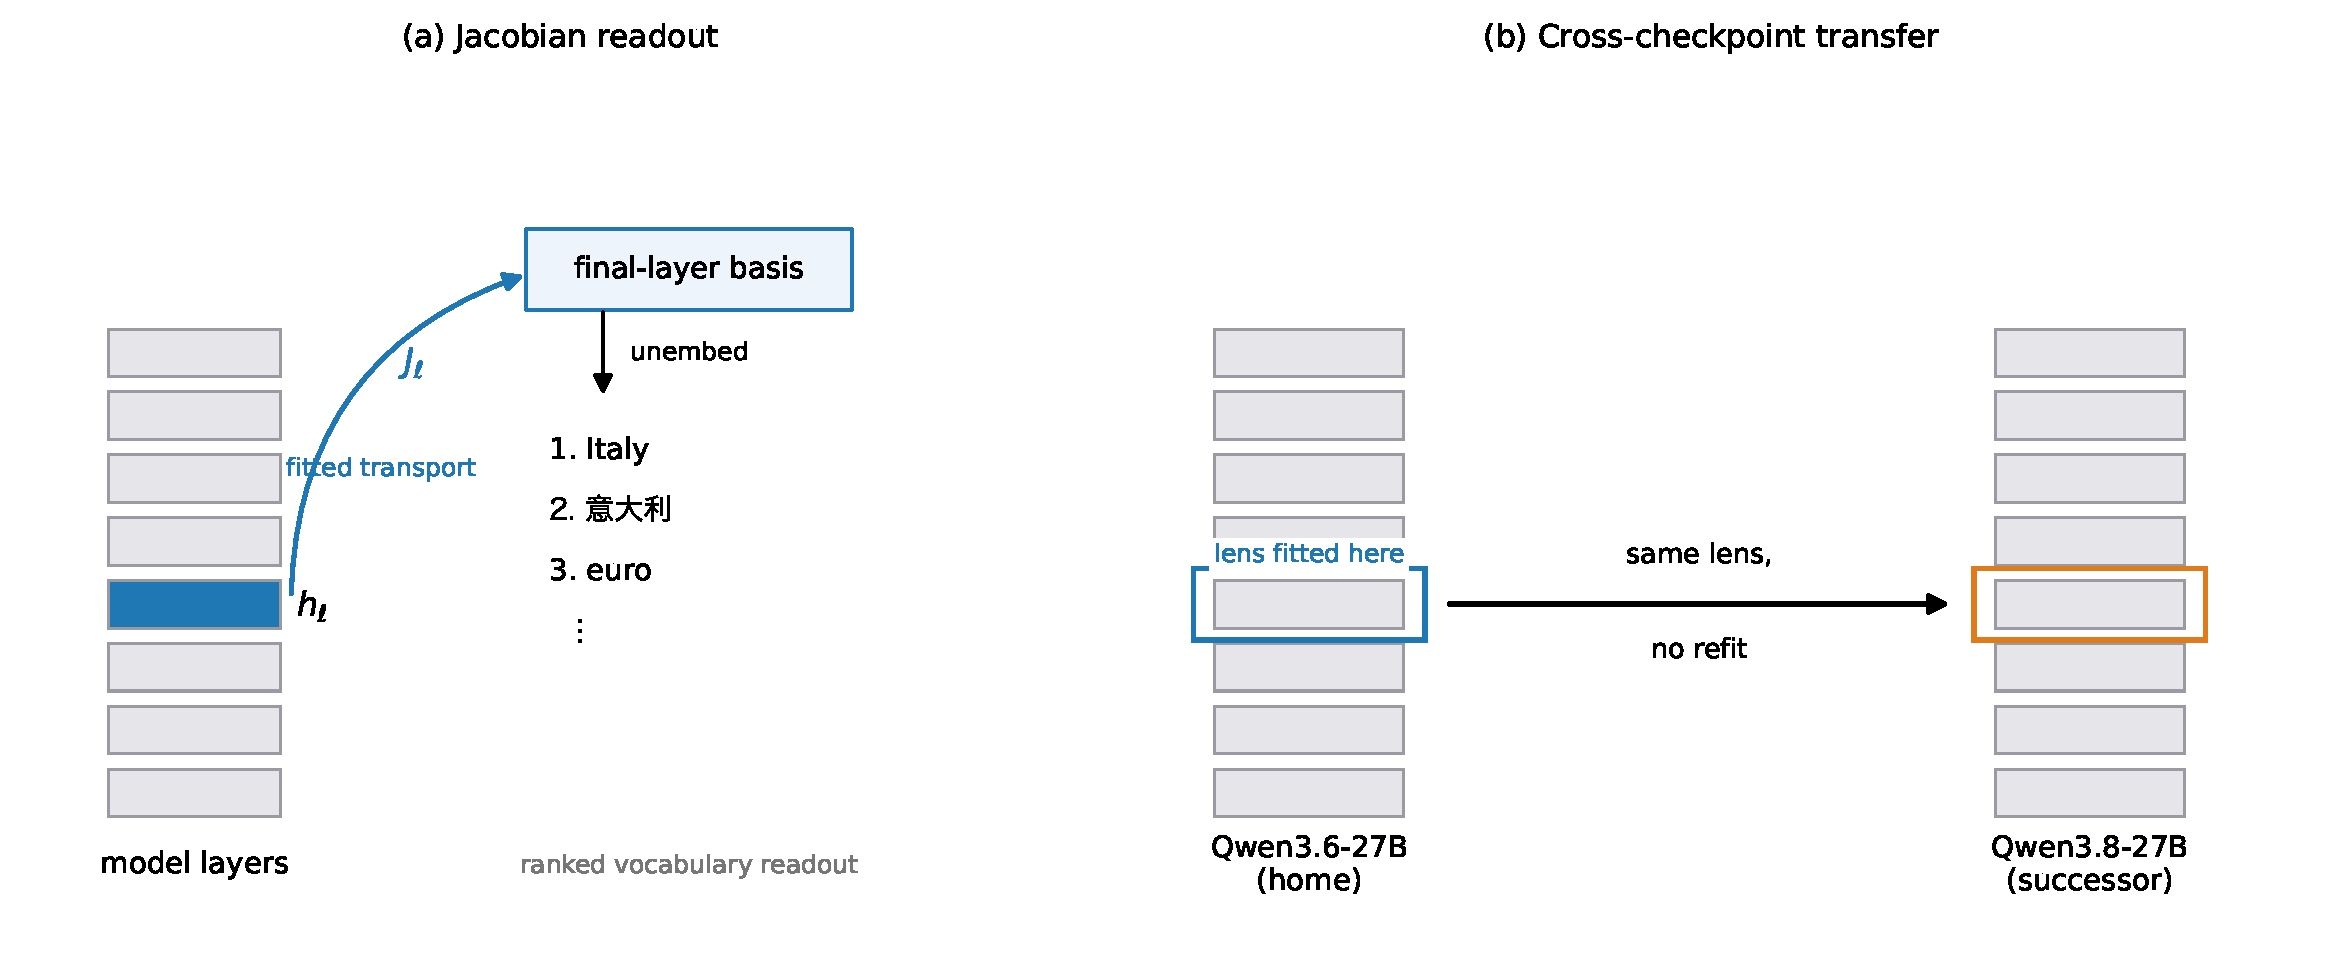
\includegraphics[width=\textwidth]{fig_concept}
\caption{The instrument and the experiment. \emph{(a)} The Jacobian readout:
a fitted per-layer transport $J_\ell$ carries an intermediate state $h_\ell$
into the final-layer basis, where the model's own unembedding yields a ranked
vocabulary readout (shown: the two-hop \emph{Italy} example).
\emph{(b)} The transfer condition tested here: the lens fitted on
Qwen3.6-27B is applied to Qwen3.8-27B without refitting.}
\label{fig:concept}
\end{figure*}

\subsection{Models, lens, and terminology}

Qwen3.6-27B and Qwen3.8-27B each have 64 layers, hidden dimension
$d_{\mathrm{model}}{=}5120$, 24 attention heads, 4 key-value heads, and a
248{,}320-token vocabulary. Both models are evaluated in bf16. We refer to
Qwen3.6-27B as the \emph{home model} and Qwen3.8-27B as the \emph{successor
model}. The published Qwen3.6-27B Jacobian lens is the \emph{home lens}; its
unchanged application to Qwen3.8-27B is the \emph{transferred lens}.

For layer $\ell$, the lens contains a transport
\[
J_\ell = \mathbb{E}\!\left[\frac{\partial h_{\mathrm{final}}}
{\partial h_\ell}\right]
\]
estimated from the home model's local geometry. We use \emph{Jacobian
readout} for vocabulary logits computed after this transport and \emph{raw
readout} for logits computed by applying the unembedding directly to the
intermediate state. These names distinguish the measured readouts from the
global-workspace interpretation considered later. Figure~\ref{fig:concept}
summarizes the readout and the transfer condition.

\subsection{Readout measure and comparisons}

At token position $p$, the Jacobian readout is
$\mathrm{unembed}(J_\ell h_{\ell,p})$ and the raw readout is
$\mathrm{unembed}(h_{\ell,p})$. The outcome is the rank assigned to a target
token among all 248{,}320 vocabulary items; rank 1 is best. We evaluate layers
$\{4,8,\ldots,60,62\}$. One script, prompt set, position set, and ranking rule
are used for all four combinations of model and readout.

Headline tables report the median target rank. Where paired tests are
reported, comparisons are made at the prompt or token-position level. Sign
tests exclude ties (the ``decided'' cases), and confidence intervals summarize
the paired $\log_{10}$ rank ratio. These comparisons measure the combined
effect of version change and home-lens mismatch; the design cannot separate
those components.

\subsection{Primary and secondary evaluation tasks}

The primary task contains 40 English two-hop prompts. Each prompt names a
property of a country and asks for another property while leaving the country
itself unstated. For example, in ``\emph{Fact: The currency used in the country
shaped like a boot is},'' the target is the first token of \emph{Italy}. The
rank is measured at the final prompt position. The set contains a limited
entity pool and repeats some targets; results therefore describe this prompt
set rather than 40 independent entities.

The secondary task uses WikiText-103 test passages
\citep{merity2016pointer}. The first 100 passages longer than 800 characters
are tokenized and truncated to 128 tokens. The teacher-forced next token is
ranked at positions 32, 48, 64, 80, 96, 112, and 126, yielding 700 position
samples per model. The task measures surface next-token readability under the
same protocol on both checkpoints. It is not directly comparable with the
published artifact-card evaluation, which uses a different protocol.

\subsection{Exploratory 35B follow-up}
\label{sec:35b-methods}

The exploratory follow-up uses a second fitted artifact, the
Qwen3.6-35B-A3B Jacobian lens released by \citet{stanley2026lens35}. It
contains transports from source layers 0--38 into layer 39 and was fitted on
1{,}000 WikiText-103 prompts. We apply it unchanged to two compatible
40-layer mixture-of-experts targets: Qwen3.5-35B-A3B Instruct in BF16
\citep{qwen35card}, and the HauhauCS Qwen3.6-35B-A3B abliterated derivative
in Q8\_K\_P \citep{hauhau2026model}. The target model's own output norm and
unembedding are used in each condition. As a decoder-identity gate, decoding
the captured final-layer state reproduces the model's next-token argmax at
every tested position on both targets. Because only the quantized HauhauCS
build was available and the follow-up does not match the full primary
protocol, its results are treated as provisional.

The latent-entity evaluation reuses the exact 40 prompts and first-token
targets from the primary 27B task. Jacobian and raw ranks are computed at the
last prompt position for all source layers. A separate surface-token check
ranks the true next token at 212 positions from one fixed encyclopedic
paragraph. Because that paragraph is not the 700-position WikiText battery
and its home-model comparator comes from the artifact documentation, it is
reported only as an order-of-magnitude check. No matched intervention was run
for the 35B targets.

\subsection{Supporting checks}
\label{sec:supporting-methods}

The causal check uses directions computed entirely from the home lens. For
token forms corresponding to \emph{paradox}, \emph{paradoxical}, and two
Chinese equivalents, the pullback directions $J_\ell^{\top}u_w$ are
orthogonalized within each layer and projected out of the residual stream at
layers 18--47 during generation and activation capture. The prompt is
``Describe Escher's impossible staircase.'' We cross model, clean versus
ablated generation, and the model's reasoning mode enabled versus disabled,
for eight cells in total. This is a one-prompt, one-concept demonstration, not
a general estimate of steering reliability.

Two further checks are exploratory. First, two behavioral prompt pairs on the
home model are resampled at temperature 0.7 and compared with greedy captures.
Second, a fixed self-description prompt with a forced completion prefix,
previously characterized on the home model, is run once on the successor with
the transferred lens at layers 39--55. These checks are reported separately
from the two quantitative tasks and are not pooled with their estimates.

\section{Results}

We first report the main model-by-readout comparisons for the two-hop
and WikiText tasks. The intervention, sampling, and held-content examples are
then presented as supporting analyses.

\subsection{Latent-entity readout}

Figure~\ref{fig:ranks} (left) shows that the home and transferred Jacobian
readouts follow a similar depth profile. Across layers 24--48, where the target
entity is most readable, the transferred lens assigns median ranks from 4 to
470. The raw readout assigns median ranks of roughly $10^3$--$10^4$ on both
models through the same band (Table~\ref{tab:ranks}).

The paired comparisons show that transfer is not uniform across depth. At
layers 44--48, the transferred lens has a higher target rank than the home
lens: median paired rank inflation is $1.7\times$ at layer 44 and $3.4\times$ at layer 48 (sign test, $p<10^{-3}$; bootstrap 90\% confidence
intervals for the median $\log_{10}$ ratio are $[+0.15,+0.38]$ and
$[+0.30,+0.65]$). Layer-40 readout is at parity ($p=0.21$). At layers 24--36,
the direction reverses. At layer 24, for example, the successor's median rank
is 38 compared with 121 on the home model; 32 of 39 non-tied prompts favor the
successor ($p<10^{-3}$), with median ratios of $0.4$--$0.7\times$ across this range.

This earlier-depth advantage has more than one possible source. It is
consistent with the successor making the target content readable earlier, but
the transfer cell changes both the underlying model and the match between
model and lens. The experiment therefore cannot attribute the difference to
one source. As a qualitative example, the transferred lens ranks
\emph{Italy} first at layer 40 on Qwen3.8-27B, with Chinese-script forms of
\emph{Italy} and \emph{euro} also in the top five. Figure~\ref{fig:board} shows the full
depth-by-position readout for this prompt on both models.

\begin{figure*}[t]
\centering
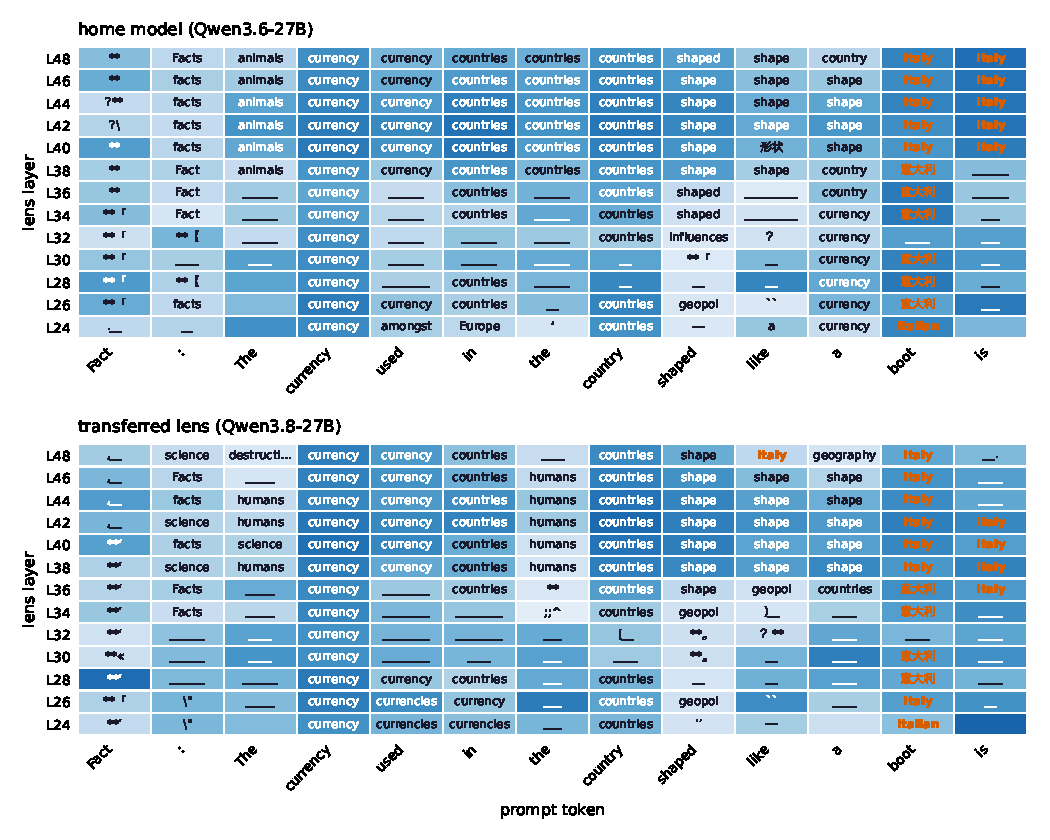
\includegraphics[width=\textwidth]{fig_board}
\caption{Transferred readout on one two-hop prompt, in the style of the
workspace paper \citep{gurnee2026workspace}. Each cell shows the top-ranked
vocabulary token of the Jacobian readout at that layer and prompt position
(prefill only); shading gives its probability mass, and orange marks the
target family (\emph{Italy}, \emph{Italian}, Chinese-script \emph{Italy}).
The unstated middle entity becomes the leading readout well before the final
position on both the home model (top) and the successor under the transferred
lens (bottom). The capture is released with the dataset.}
\label{fig:board}
\end{figure*}


\begin{figure*}[t]
\centering
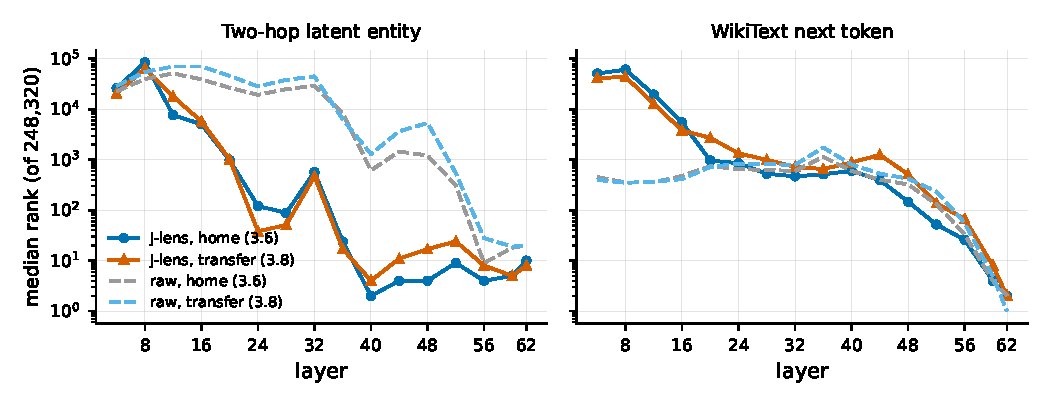
\includegraphics[width=\textwidth]{fig_ranks}
\caption{Median target-token rank by evaluation layer on a log scale. Lower
is better. \emph{Left}: the unstated intermediate entity in 40 two-hop
prompts. \emph{Right}: the teacher-forced next token at 700 WikiText
positions. ``Home'' applies the Qwen3.6-27B lens to Qwen3.6-27B; ``transfer''
applies the same lens without modification to Qwen3.8-27B. ``Raw'' applies
the unembedding without Jacobian transport.}
\label{fig:ranks}
\end{figure*}

\begin{table*}[t]
\centering
\scriptsize
\setlength{\tabcolsep}{4.2pt}
\begin{tabular}{@{}r rrrr rrrr@{}}
\toprule
& \multicolumn{4}{c}{Two-hop latent entity} &
  \multicolumn{4}{c}{WikiText next token}\\
\cmidrule(lr){2-5}\cmidrule(lr){6-9}
& \multicolumn{2}{c}{home model} & \multicolumn{2}{c}{successor model} &
  \multicolumn{2}{c}{home model} & \multicolumn{2}{c}{successor model}\\
\cmidrule(lr){2-3}\cmidrule(lr){4-5}\cmidrule(lr){6-7}\cmidrule(lr){8-9}
layer & J-lens & raw & J-lens & raw & J-lens & raw & J-lens & raw\\
\midrule
 8 & 84{,}539 & 39{,}620 & 63{,}868 & 54{,}560 & 60{,}810 & 353 & 43{,}645 & 349\\
16 & 5{,}042 & 38{,}980 & 5{,}739 & 70{,}285 & 5{,}486 & 477 & 3{,}798 & 413\\
24 & 121 & 19{,}219 & 38 & 28{,}224 & 852 & 654 & 1{,}339 & 832\\
32 & 570 & 29{,}185 & 470 & 44{,}822 & 468 & 601 & 719 & 791\\
40 & 2 & 617 & 4 & 1{,}299 & 600 & 603 & 881 & 802\\
48 & 4 & 1{,}213 & 17 & 5{,}341 & 147 & 323 & 514 & 421\\
56 & 4 & 9 & 8 & 28 & 26 & 33 & 67 & 56\\
62 & 10 & 20 & 8 & 20 & 2 & 2 & 2 & 1\\
\bottomrule
\end{tabular}
\caption{Median target-token rank for selected layers. The two-hop task uses
40 prompts at the final prompt position; the WikiText task uses 700
teacher-forced position samples per model. J-lens denotes the Jacobian
readout. Raw denotes direct unembedding of the intermediate state.}
\label{tab:ranks}
\end{table*}

\subsection{Surface next-token readout}

The WikiText comparison shows a smaller but consistent transfer penalty
(Figure~\ref{fig:ranks}, right). At mid-network layers, paired per-position
rank inflation is $1.2$--$1.3\times$ (layer 32:
$p=3\times10^{-5}$). By layer 48 it is approximately $2\times$
($p<10^{-30}$, $n{=}700$). The raw readout shifts by a similar factor at mid-network layers ($1.2$--$1.3\times$ at layers 24--40), so the mid-network inflation is not specific to the lens; the lens-specific cost is concentrated at layer 48, where the Jacobian readout inflates $2.0\times$ against $1.2\times$ for the raw readout (Table~\ref{tab:ranks}).

Thus the two tasks show different transfer profiles: latent-entity readout
remains close to the home condition over its strongest band, whereas
next-token readout shows a clearer late-layer cost. One interpretation is
that version training changed directions involved in fine-grained token
prediction more than those used by the latent-entity readout. Because the
experiment does not isolate lens mismatch from model change, this remains an
interpretation rather than a direct measurement of the training update.

\subsection{Exploratory 35B latent-entity result}
\label{sec:35b-results}

The central latent-entity pattern also appears in the exploratory 35B
measurements (Table~\ref{tab:35b}). At the six summary layers from 20 to 38, the
transferred Jacobian readout keeps the median target at or below rank 15.5 on
both targets. On Qwen3.5-35B-A3B Instruct, the median best rank across the
stack is 3 and 14 of 40 targets reach rank 1 somewhere in the stack. On the
HauhauCS derivative, the corresponding values are 2 and 18 of 40. The raw
readout is three to four orders of magnitude worse at layers 20--28 and
catches up only near the output.

\begin{table}[t]
\centering
\scriptsize
\setlength{\tabcolsep}{3pt}
\resizebox{\columnwidth}{!}{%
\begin{tabular}{@{}r rr rr@{}}
\toprule
& \multicolumn{2}{c}{Qwen3.5-35B Instruct} &
  \multicolumn{2}{c}{HauhauCS Qwen3.6-35B} \\
\cmidrule(lr){2-3}\cmidrule(lr){4-5}
layer & J-lens & raw & J-lens & raw \\
\midrule
20 & 6.5  & 3{,}415 & 4.5 & 2{,}550 \\
24 & 14   & 5{,}934 & 3   & 1{,}598 \\
28 & 15.5 & 9{,}699 & 14  & 5{,}614 \\
32 & 5.5  & 52.5    & 4   & 27.5 \\
36 & 11.5 & 23      & 9   & 19 \\
38 & 8    & 28.5    & 7   & 18.5 \\
\bottomrule
\end{tabular}}
\caption{Exploratory 35B follow-up on the same 40 two-hop prompts. Entries
are median first-token target ranks (lower is better) for the
Qwen3.6-35B-A3B lens applied unchanged. The protocol reports the
latent-entity evaluation only.}
\label{tab:35b}
\end{table}

The separate 212-position surface-token check is also of the same order as
the lens artifact's home-model documentation at layers 8, 16, 24, and 32,
but the corpus and position protocol are not matched. We therefore use it as
a calibration check rather than evidence for a quantitative transfer
penalty. These provisional measurements show a similar latent-entity pattern
with a second fitted lens and two related targets. They motivate a fully
matched 35B replication but do not establish one.

\subsection{Supporting analyses}

\paragraph{Single-concept intervention.}
In all four clean cells, the generated descriptions contain the word
\emph{paradox}, and the lens assigns the paradox token group a pooled band
mass of 124--157. In all four ablated cells, the word is absent and the
corresponding readout is zero. The descriptions remain coherent and preserve
the same central details, including the lithograph, closed loop, and illusion.
Neighboring concepts such as \emph{illusion} and \emph{impossible} decrease
two- to three-fold in the captured field but remain present in the text.
Within this prompt and concept, directions computed from the Qwen3.6-27B lens
therefore affect both the Qwen3.8-27B readout and its generated wording. The
result supports transfer of this intervention but does not estimate how often
such transfer will hold for other concepts or prompts.

\paragraph{Sampling check on the home model.}
At temperature 0.7, the surface wording changes across the two behavioral
prompt pairs, while the leading never-generated words in the deep-band
readout (words that rank highly in the readout but do not appear in the
generated text) retain their identities and nearly the same ordering. Per-word mass
varies by approximately a factor of two. In the verbatim-copy control, the
sampled output is token-identical to the greedy output, and the capture also
matches. This small check is consistent with local sampling stability, but it
contains only two prompt pairs and does not test the successor model.

\paragraph{Exploratory held-content example.}
In the fixed self-description prompt, affect terms such as \emph{feels} and
\emph{feelings} are among the strongest words read at layers 39--55 but do not
appear in the generated output. The same qualitative signature had been
observed on the home model. This example suggests that a previously observed
form of latent--verbal divergence can also be found with the transferred lens.
Because it is a single fixed prompt selected from earlier work, it is an
illustration rather than an estimate of prevalence. The released capture
contains the full field.

\section{Discussion}

\subsection{What transfers in this experiment}

The primary result is functional: a Jacobian lens fitted to Qwen3.6-27B
continues to recover the target entity when applied unchanged to Qwen3.8-27B.
Over the layers where the entity is most readable, the transfer cost is
bounded to small rank factors and the readout remains much stronger than the
raw baseline. The WikiText task shows that transfer is not cost-free; its
penalty grows near the output end of the network. The intervention provides
additional, narrower evidence that at least one direction derived from the
home lens remains behaviorally relevant on the successor.

The exploratory 35B follow-up yields a similar latent-entity pattern with a
second fitted artifact and a mixture-of-experts architecture. Because one
target is available only after Q8\_K\_P quantization, and because the
follow-up does not match the WikiText protocol or repeat the intervention,
it is a lead for replication rather than independent corroboration of the
primary study.

These findings are compatible with partial stability of the verbalizable
representational basis proposed by \citet{gurnee2026workspace}. They are not a
direct measurement of basis conservation. Similar readout performance can
arise despite internal changes, and both fitted artifacts are tested only
within related Qwen checkpoints or derivatives.

\subsection{Implications for monitoring}

Cross-checkpoint transfer can be treated as a measurable property rather than
an assumption. For the matched 27B version step, the existing lens remains
useful enough to compare selected readouts without first fitting a
replacement. The provisional 35B result makes broader testing across fitted
artifacts worthwhile but does not establish generality. Repeating the same
transfer test at later releases would reveal when an instrument begins to
drift or fail. The results therefore support the possibility of amortizing
lens-fitting costs within a model line, but they are not sufficient to
establish a once-per-line fitting rule.

\subsection{Alternative explanations}

The matched architecture and tokenizer may be important conditions for the
observed transfer. The undocumented training relationship may also range from
continued training of a shared base to a more complicated reuse of weights or
data. In addition, the successor's better ranks at some middle layers cannot
be assigned uniquely to earlier content resolution, because both model state
and lens fit differ between the home and transfer conditions. A design with
newly fitted lenses on both checkpoints, or additional intermediate releases,
would help separate these explanations.

The 35B targets add further confounds: one is an older Instruct checkpoint,
whereas the other is an abliterated derivative evaluated after Q8\_K\_P
quantization. Their comparison does not isolate version, post-training, or
quantization effects. The exploratory result is therefore evidence of
operational readout under those combined changes, not an estimate of any one
change's effect.

\section{Related Work}

\paragraph{Vocabulary-space readouts.}
The Jacobian lens was introduced by \citet{gurnee2026workspace}, with
reference code and fitted lenses released for several open models
\citep{neuronpedia2026lens}. Community-fitted artifacts now include a
397B-parameter mixture-of-experts model \citep{praxagent2026lens397}.
\citet{wu2026jcot} subsequently use J-space as a recurrent interface for
chain-of-thought. These studies motivate the practical question addressed
here: whether an already fitted Jacobian lens remains usable after its model
line is updated.

\paragraph{Comparing checkpoints.}
Model diffing commonly trains a shared object, such as a crosscoder, across
two checkpoints to expose their differences \citep{lindsey2024crosscoders}.
The present test asks a complementary and narrower question. It does not
train a representation across the pair; it measures how an existing
instrument's readout changes when moved from one checkpoint to another.

\paragraph{Latent and verbalized content.}
Chain-of-thought can be an incomplete or unreliable account of the
computation accompanying an answer \citep{lanham2023faithfulness,
arcuschin2025faithful}. Vocabulary-space readouts offer a different view of
intermediate content. Their value for monitoring successive model versions
depends in part on whether changes in the readout can be distinguished from
failures of the instrument itself, which is the stability question tested
here.

\section{Limitations}
\label{sec:limits}

The study has six main boundaries. First, it tests one interpretability
method, one fitted artifact in a matched transfer study, and a second artifact
in an exploratory follow-up. Every source and target remains within the Qwen
family and each transfer uses a compatible architecture and tokenizer. It
does not establish transfer across model families, incompatible
architectures, or larger version gaps.

Second, the same 40 English two-hop prompts are reused across the 27B and 35B
tests. They draw from a limited entity pool with repeated targets and score
only the target entity's first token. The 700 WikiText observations in the
primary study come from fixed positions within 100 passages and should not be
treated as 700 independent documents.

Third, the 35B follow-up does not match the full primary protocol. Its
surface-token check uses one 212-position paragraph, one target is quantized
and abliterated, and no matched causal intervention was run. The follow-up
therefore motivates replication of the latent-entity result but does not
itself support a replication claim.

Fourth, the main runs are greedy and single-seed. The temperature check
covers only two prompt pairs on the 27B home model, so it cannot establish
general sampling stability. The held-content result is likewise a selected,
single-prompt qualitative example. Fifth, the causal check uses one concept,
one prompt, and one intervention band, with no dose-response curve or broader
prompt set. It demonstrates an effect in those cells but does not bound the
generality or specificity of the intervention.

Finally, the transfer condition changes the model and the lens--model match at
the same time. Paired tests localize and bound their combined effect, but they
do not determine how much is caused by representational change in the
successor and how much is caused by lens misfit. Any claim that the underlying
workspace basis itself was conserved is therefore an inference from readout
behavior, not a separately identified result.

\section{Conclusion}

This study answers its operational research question with a qualified no: a
fitted lens need not always be refitted after a nearby,
architecture-compatible model update. Applied unchanged to Qwen3.8-27B, the
Qwen3.6-27B lens retained the unstated-entity signal (median rank 4 at home, 17
after transfer, and 5{,}341 in the successor's raw readout), and its
\emph{paradox} directions still altered both readout and generation. Yet the
layer-dependent WikiText errors show that useful transfer did not preserve
the lens's original calibration.

Cross-checkpoint reuse is therefore an empirical calibration problem, not a
choice between assuming portability and refitting by default. For longitudinal
interpretability and alignment monitoring, a lens can be carried forward when
validation at the relevant layers, tasks, and targets shows that it remains
fit for purpose. Measuring transfer error enables reuse while guarding against
mistaking lens--model mismatch for change in the model. The decisive next step is to fit a Qwen3.8-27B lens, compare old-on-old, old-on-new, and new-on-new readouts, and expand the intervention across releases and concepts. That would separate model drift from instrument error and support an empirical threshold for refitting.

\section*{Reproducibility}

Evaluation code, the two-hop prompt set, per-layer rank tables for all four
model-by-readout cells, and the exploratory capture are available at
\url{https://huggingface.co/datasets/ec75hash/jacobian-lens-transfer-qwen36-38}.
The exploratory 35B follow-up is in the same dataset under \path{exploratory_35b/}: the two per-target S1/S2 result files, the exact prompt set, decoding and capture code, run logs, and a provenance note with the recorded model and lens hash prefixes.

\section*{AI Collaboration Statement}

This paper was prepared with AI assistance. Claude (Anthropic) drafted
evaluation code and earlier prose; OpenAI Codex assisted with manuscript
revision and typesetting under the author's direction. All experiments,
claims, and final text were reviewed and are the responsibility of the human
author. Every reference was verified against its source.

\bibliographystyle{plainnat}
\bibliography{refs_revised}

\end{document}
